% THIS IS AN EXAMPLE DOCUMENT FOR VLDB 2010
% based on ACM SIGPROC-SP.TEX VERSION 2.7
% Modified by  Gerald Weber <gerald@cs.auckland.ac.nz>


% This example *does* use the .bib file (from which the .bbl file
% is produced). REMEMBER HOWEVER: After having produced the .bbl file,
% and prior to final submission, you need to 'insert'  your .bbl file into
% your source .tex file so as to provide ONE 'self-contained' source file.


\documentclass[a4paper,12pt]{report}
\renewcommand{\baselinestretch}{1.5}
%\usepackage[linesnumbered,boxed]{algorithm2e}
\usepackage{amsmath}
\usepackage{amsthm}
\usepackage{algorithm}
\usepackage{algorithmic}
%\usepackage{algpseudocode}
\usepackage{graphicx}
\usepackage{verbatim}
\usepackage{latexsym}
\usepackage{subfigure}
\usepackage{subfig}
\usepackage{color}

\usepackage{float}
\usepackage{indentfirst}
\usepackage{wallpaper}
\usepackage{pdfpages}
\usepackage{multirow}
\newtheorem{theorem}{Theorem}
%\usepackage{pdfpages}
%\usepackage{hyperref}
\usepackage{CJK}

\CenterWallPaper{.30}{figure/nthu-logo.pdf}

%set paper size
\special{papersize=8.5in,11in}
\topmargin=14.7mm    %bottom margin 14.7mm
\oddsidemargin=30mm   %left & right margin 17.45mm

%text sizes (Keep these values unchanged!)
\textwidth=150mm \textheight=250mm
\columnsep=5.0mm
\parindent=3.5mm

%misc parameters
\headsep=0mm  \headheight=0mm \footskip=18mm

%conversion to values for LaTeX
\advance\topmargin-1in\advance\oddsidemargin-1in
\evensidemargin\oddsidemargin


\begin{document}

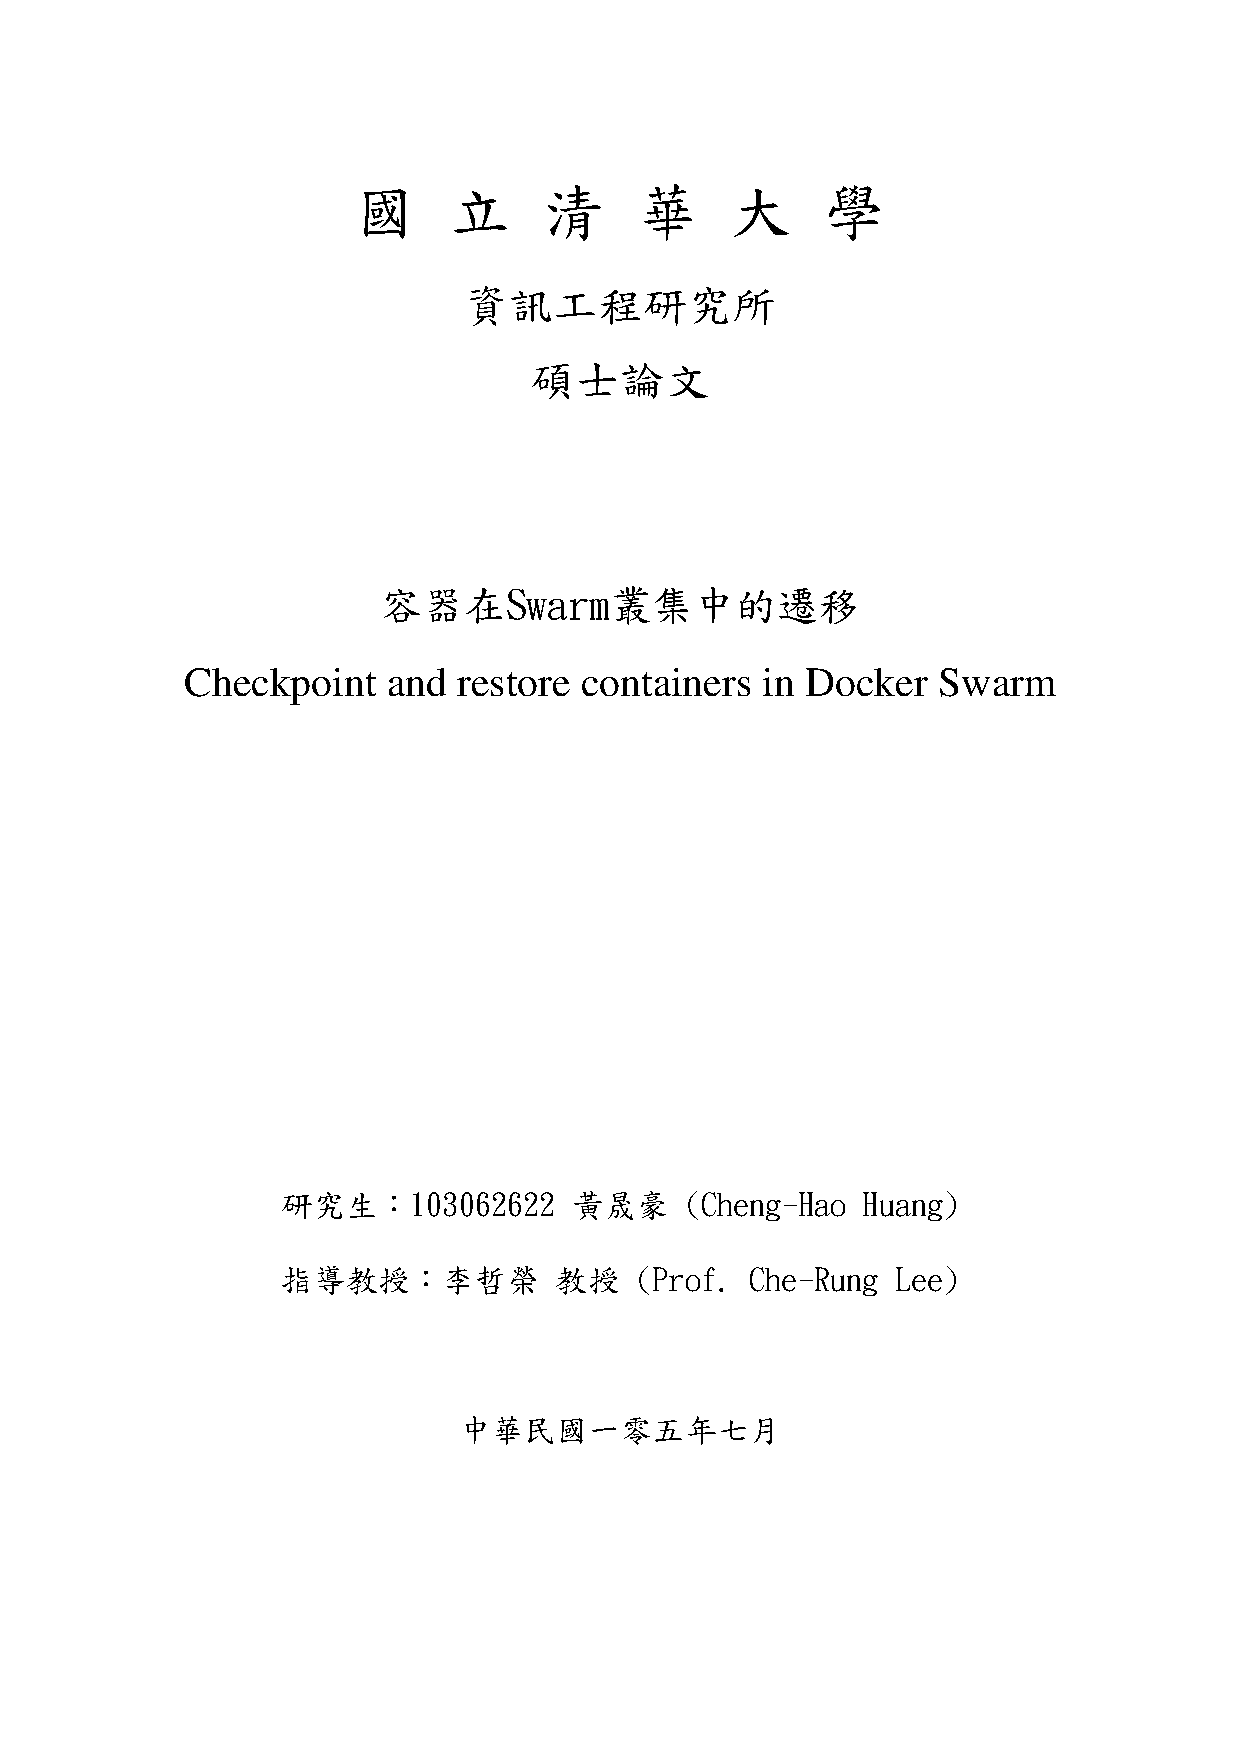
\includepdf[pages={1}]{cover.pdf}
%\includepdf[pages={1}]{cover_ch.pdf}

\title{\bf \huge Docker containers migration in Docker swarm}
\date{}
\author{
\begin{tabular}{c}
\\
\\
{\LARGE \bf Student: Cheng-Hao Huang}\\
{\LARGE \bf Advisor: Prof. Che-Rung Lee}\\
\\
\\
\\
\\
{\LARGE \bf Department of Computer Science}\\
{\LARGE \bf National Tsing Hua University}\\
{\LARGE \bf Hsinchu, Taiwan, 30013, R.O.C.}\\
\\
{\large July 2016}
\end{tabular}
}

\maketitle
\includepdfset{pagecommand={\thispagestyle{plain}}}

\pagenumbering{roman}
%\addcontentsline{toc}{chapter}{\ctxfr 中文摘要}
\addcontentsline{toc}{chapter}{Chinese Abstract}

\includepdf[pages={1}]{abstract_ch.pdf}

\addcontentsline{toc}{chapter}{Abstract}
\begin{abstract}
\thispagestyle{plain} 
\setcounter{page}{2}

Container becomes a popular technology since Docker has published in 2013.
Container technology has solved programmer and system maintainer when they have to deploy their applications in the servers.
They just need to build the container images, and the container images can run on everywhere they want.
Container technology also isolates each container environments just likes a single host machine.

In this paper, we not only migrate the Docker containers between two physical machines, but also migrate the Docker containers in the Docker Swarm cluster.
Furthermore, we enhance the high availability in the Docker Swarm cluster, the container can be set that checkpoint the container images to remote storage service; whenever the Docker Nodes are fail, the containers which run in the failed Docker Nodes will restore the newest checkpoint to the alive Docker Nodes as well.
\end{abstract}



\addcontentsline{toc}{chapter}{Acknowledgements}
\renewcommand{\abstractname}{Acknowledgements}
\begin{abstract}
\thispagestyle{plain}
\setcounter{page}{3}


\end{abstract} 

\setcounter{page}{4}
\addcontentsline{toc}{chapter}{Contents}
\tableofcontents
\clearpage
\addcontentsline{toc}{chapter}{List of Figures}
\listoffigures
\clearpage
\addcontentsline{toc}{chapter}{List of Tables}
\listoftables
\clearpage
\addcontentsline{toc}{chapter}{List of Algorithms}
\listofalgorithms
\clearpage


\pagenumbering{arabic}
\setcounter{page}{1}
\chapter{Introduction}
\label{chap:intro}
Traditionally, people rely single supercomputer to calculate data or deploy their companies' application. Nowadays, cloud computing has been use wildly. People would like to use a lot of normal computers that gather them into a cluster to replace a supercomputer. More and more companies build their data centres or use cloud platforms to construct their business application.
However, the more computers we have, the more power consumption problem we have to solve. At the same time, to make sure every computers' process in the cluster are alive, high availability becomes a more important role in cloud computing.

Virtualization is a popular technology that is used wildly on cloud computing,  including virtual operating system, computer hardware platforms, storage device and computer network resources.
Virtual machine is a technology to emulate a particular computer like a real computer. It can partition a physical machine resource, such as CPU, memory, storage, and network.
A hypervisor uses execution to manage and share host physical machine hardware, it allows many different virtual machines isolated from each other.

Container is operating system level virtualization which runs as an isolated process in userspace on the host operating system and shares the same operation system kernel with other containers.
It provides kernel namespace such as PID, IPC, network, mount, and user namespace to isolate each container environment to host operation system.
In order to control hardware resource like CPU, memory, network, and disk I/O, container uses cgroups to limit each container resources.
Container doesn't have hypervisor to isolate with host operating system, therefore, it can offer better performance than virtual machine. It already has many software to control container, like LXC \cite{helsley2009lxc}, LXD, Open VZ, For now, Docker \cite{Docker} is the most popular container engine. The Virtual Machine and Container architecture is shown as Fig \ref{fig:VM_vs_container}.

\begin{figure}[h]
\begin{center}
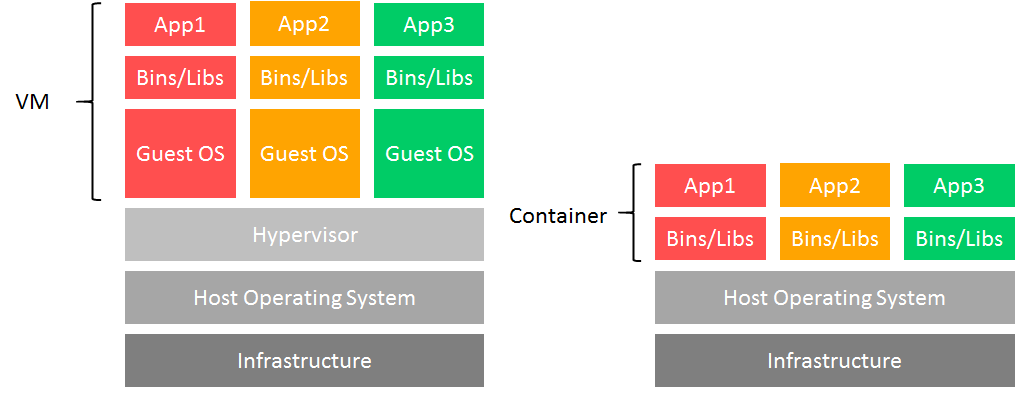
\includegraphics[width=15cm]{figure/VM_vs_container.png}
\end{center}
\caption{Virtual Machine and Container architecture}
\label{fig:VM_vs_container}
\end{figure}

Checkpoint and restoration can freeze a running process state and save process information to checkpoint images. User can use these checkpoint image files to restore the process which user want to restore the process state. These features can be used to dump checkpoint and restore containers because each containers are processes in the host operating system.

In this paper, we choose container but not Virtual Machine to do migration between two host machines, because container need less disk storage and less network transport resources. We not only use checkpoint and restoration to migrate the containers between two physical computers but also migrate the containers in the Docker cluster.
There are many Docker cluster software, like Docker Swarm, Google Kubernetes, Apache Mesos, etc. We choose Docker Swarm because it support native Docker API, and Docker usage habit. We don't need to learn the other Docker cluster software.
Moreover, we improve high availability and rescheduling feature in Docker Swarm using checkpoint and restoration than keep versions of container checkpoint images in remote storage server that whenever computer are fail, Docker Swarm manager will restore the containers from the checkpoint images.

\chapter{Background}
\label{chap:background}
\section{Docker}
Docker is a open-source project container engine. It provides an additional layer of abstraction and automation of operating-system-level virtualization on Linux. Docker engine include Docker client and Docker daemon.
\subsection{Docker client}
Docker is typical Client/Server architecture application. Docker client uses Docker command to send and receive requests to Docker daemon. Also, Docker supports remote RESTful API to send and receive HTTP requests to Docker daemon, it has been implemented by more than 10 programming languages.
\subsection{Docker daemon}
Docker daemon is a daemon that runs as system service. It has two the most importance features: 
\begin{itemize}
    \item Receive and handle Docker client's requests.
    \item Manage containers.
\end{itemize}
When docker daemon is running, it will run a server that receives requests from Docker clients or remote RESTful API. After receives requests, server will pass requests by router to find handler to handle the requests.
\section{Docker Swarm}
Docker Swarm is native clustering for Docker. It gathers several docker engines together into  one virtual docker engine. Docker Swarm serves standard Docker API, so it can be connected by Dokku, Docker Machine, Docker Compose, Jenkins, DockerUI, Drone, etc. And it also support Docker client of course.
In Docker Swarm, It has two components, Include Swarm master and Swarm node. Swarm master is the manager which handles Docker client and RESTful API requests and manages multiple Docker nodes resources. Docker node is an agent which sends heartbeat to discovery server to ensure Docker daemon is alive in the cluster.
\subsection{Discovery services}
Docker Swarm provides multiple discovery services backends. They are used to discovery nodes in the cluster. There are:
\begin{itemize}
    \item Using a distributed key/value store, like Consul, Etcd and Zookeeper.
    \item A static file or list of nodes.
    \item Docker Hub as a hosted discovery service
\end{itemize}
Otherwise, It also supports any modules which satisfy discovery API interface.
\subsection{Scheduler}
Docker Swarm scheduler decides which nodes to use when creating and running a container. It has two steps. First, It follows user's filters to decide which nodes are conform. Second, It passes through strategies to select the best node in the cluster.
\subsubsection{Filter}
Filters are divided into two categories, node filters and container configuration filters. Node filters operate on characteristics of the Docker host or on the configuration of the Docker daemon. Container configuration filters operate on characteristics of containers, or on the availability of images on a host.
The node filters are:
\begin{itemize}
    \item constraint
    \item container slots
    \item health filter
\end{itemize}
The container configuration filters are:
\begin{itemize}
    \item affinity
    \item dependency
    \item port filter
\end{itemize}
\subsubsection{Strategies}
The Docker Swarm scheduler features multiple strategies for ranking nodes. Swarm currently supports these values:
\begin{itemize}
    \item spread
    \item binpack
    \item random
\end{itemize}
Spread and binpack strategies compute rank according to a node’s available CPU, its RAM, and the number of containers it has. It selects a node at random. Under the spread strategy, Swarm optimizes for the node with the least number of containers. The binpack strategy causes Swarm to optimize for the node which is most packed. The random strategy uses no computation, chooses nodes at random regardless of their available CPU or RAM.
\subsection{High availability}
In Docker Swarm, Swarm manager responses the cluster and manages the resources of multiple Docker nodes at scale. If Swarm master dies, we have to create a new one and deal with the interruption of service.
The High availability feature allows Docker swarm has multiple Swarm manager instances. We can create a primary manager and multiple replica instances. If we send requests to replica instances, it will be automatically proxied to the primary manager. In addition, if the primary manager fails, the others replica instances will lead a new primary manager.
\section{CRIU}
CRIU stands for Checkpoint and Restore in User Space, creates a complete snapshot of the state of a process, including things like memory contents, file descriptors, and even open tcp connections. It can be used for suspending and resuming processes, or live migrating them from one machine to another.

\ref{chap:background} and cite test \cite{Knight:1986:AMF:319838.319854, Sohi:1995:MP:225830.224451, Hammond:1998:DSS:291069.291020}.
\chapter{Conclusion}
\label{chap:conclusion}
CRIU provides the container for dumping checkpoint and restoring in the same Docker Daemon. In this thesis, we have purposed it to expand to Docker Swarm in the cluster.


\bibliographystyle{plain}
\bibliography{note}

% The following two commands are all you need in the
% initial runs of your .tex file to
% produce the bibliography for the citations in your paper.
%{%\scriptsize
%\bibliographystyle{abbrv}
%\bibliography{HPCoC_cite}
%}
% You must have a proper ".bib" file
%  and remember to run:
% latex bibtex latex latex
% to resolve all references

\end{document}
